\section{MODELLING OF THE ECRH BEAM}
\subsection{Calculation of the integration coefficients}
\normalsize{The issue was in the parameters of the \acrshort{ECRH} beam load distribution since it was not clearly defined in the recalculation task requested by Torsten Stange. The little information about the parameters of the beam load were the nominal total heat flow of 912W, Gaussian shape of power distribution and the geometric properties of both axisymmetric and non-axisymmetric distribution. Based on these data, a series of calculations aiming to recalculate the load distribution on the tile surface  were undergone and provided good results.}
\begin{figure}[h!]
    \label{fig_4_1} 
    \centering
    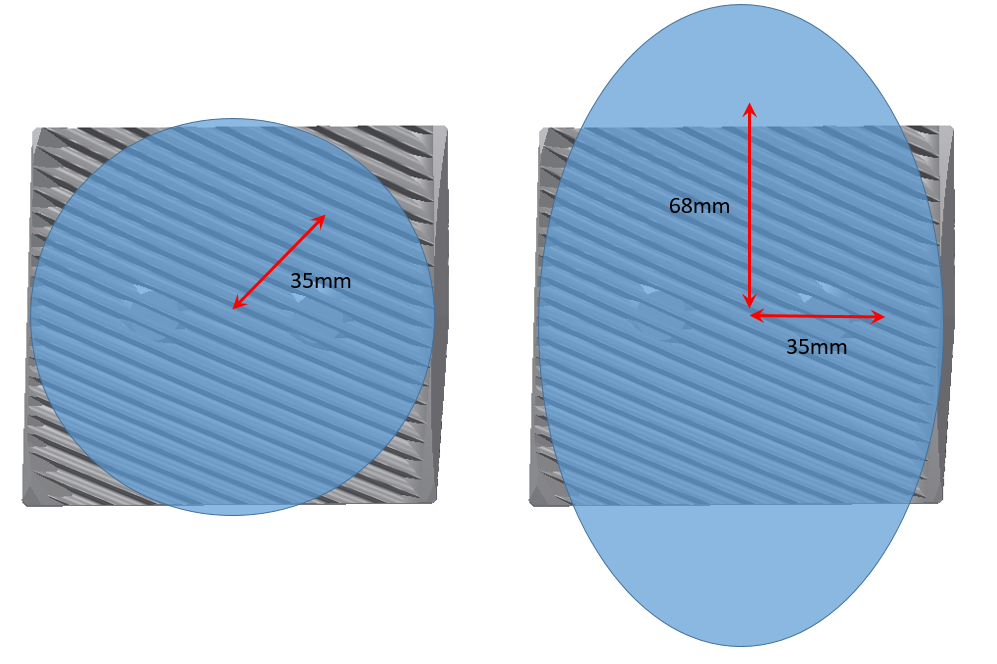
\includegraphics[width=.9\textwidth]{figures/TWOBEAMDISTRI.png}
    \caption{\it Representation of the two ECRH beam heat flux distribution cases}
\end{figure}
\\
\normalsize{\indent The calculation of the integral parameters as well as the analytical calculation of the surface integrals were done on Wolfram Mathematica\textsuperscript{\textregistered}. There are two different cases, one axisymmetric (circular) and another non-axisymmetric (elliptical). For the first case, almost all of the power ~99\% hits the ECRH reflector tile. The standard deviation is defined to be 35mm, for debug and validation purposes, 86\% of the power should be included within a disk of radius 35mm. For the elliptical distribution, much less power hits the reflector tile. The distribution properties are also different and feature two different radii, the minor semi-radius and the major semi-radius. Their values are respectively 35mm and 68mm, both of them defining an ellipse. Similarly to the circular distribution, for debugging, 86\% of the overall power should be included within the area of the ellipse.}
\\
\break
\normalsize{\indent With help of those information, the integration coefficients could be calculated. The first integral was expressed in a cylindrical coordinate system. The first APDL code written by J. Zhu \cite{zhu_parametric_2019} in 2019 only featured the circular heat flux distribution and was based on calculations made by Torsten Stange. The integrated function for Gaussian distribution has the form $\exp(-2r^2)$. The surface integral can be written:}
\\
\begin{equation}
    \int\displaylimits_{\Omega} \exp(-2r^2) \ dS \
\end{equation}
\\
\normalsize{in cylindrical coordinates, \it{$dS = rdrd\theta$}}
\normalsize{and $\Omega$ a surface in $\mathbb{R}^2$. When taking the normal distribution, is it possible to rewrite the function and include the standard deviation $r_0$. The integral $\mathbb{I}$ of $f$ on $\Omega$ is:}
\\
\begin{equation}
    \mathbb{I}_{\Omega}^f = \int\displaylimits_{\Omega} \exp\left(-2\left(\frac{r}{r_0}\right)^2 \right) \,dS
    \label{eqn:4.2}
\end{equation}
\\
\normalsize{When developing the differential (in cartesian coordinates), the integral becomes:}
\\
\begin{equation}
    \int\displaylimits_{\Omega} \exp\left(-2\left(\frac{r}{r_0}\right)^2 \right) \,dS = \int\displaylimits_0^{+ \infty} \int\displaylimits_0^{2 \pi} \exp\left(-2\left(\frac{r}{r_0}\right)^2 \right) \,rdrd\theta
\end{equation}
\\
\begin{equation}
    \int\displaylimits_0^{+ \infty} \int\displaylimits_0^{2 \pi} \exp\left(-2\left(\frac{r}{r_0}\right)^2 \right) \,rdrd\theta = \int\displaylimits_0^{+\infty} \exp\left(-2\left(\frac{r}{r_0}\right)^2 \right) \ rdr \int\displaylimits_0^{2 \pi} \ d \theta
\end{equation}
\\
\begin{equation}
    = 2 \pi \int\displaylimits_0^{+\infty} \exp\left(-2\left(\frac{r}{r_0}\right)^2 \right) \ rdr
\end{equation}
\\
\normalsize{When calculated, the value of this integral is:}
\\
\begin{equation}
    2 \pi \int\displaylimits_0^{+\infty} \exp\left(-2\left(\frac{r}{r_0}\right)^2 \right) \ rdr = 6,125 \cdot 10^{-4} \pi
\end{equation}
\\
\normalsize{\indent This function is then normalized by multiplying both side by a coefficient $k_{norm}$ such as $k_{norm} \cdot 6,125 \cdot 10^{-4} \pi = 1$ This coefficient has a value of $519,69 \ m^{-2}$. Since heat flux is in $[Wm^{-2}]$, $k_{norm}$ needs to be in $[m^{-2}]$.  To validate the normalization, it is possible to integrate the same function, but only for the radius between 0 and standard deviation and multiplying the function by $k_{norm}$. This gives:}
\\
\begin{equation}
    k_{norm} \left[ \int\displaylimits_0^{r_0} \int\displaylimits_0^{2 \pi} \exp\left(-2\left(\frac{r}{r_0}\right)^2 \right) \,rdrd\theta \right] = 0,8646
\end{equation}
\\
\normalsize{\indent The integral power of the ECRH beam is 912 W. This means that normalized ECRH beam power distribution can be multiplied by the integral power. It is thus possible to define $q_0 \coloneqq P_{ECRH}^{beam} \cdot k_{norm}$. In the case of the circular ECRH Gaussian heat flux distribution, the value of $q_0=473957 \ Wm^{-2}$, this value will be used in the APDL code. The implemented function is, in cylindrical coordinates \eqref{eqn:cylCSGHD}:}
\\
\begin{equation}
    f_{axisym.}^{cyl. CS}(r) = P_{ECRH}^{beam} k_{norm} \exp\left(-2\left(\frac{r}{r_0}\right)^2 \right) [W/m^2]
\end{equation}
\\ 
\begin{equation}
    \color{red}\boxed{\color{black} f_{axisym.}^{cyl. CS}(r) = 473957 \exp\left(-2\left(\frac{r}{35[mm]}\right)^2 \right) [W/m^2]}
    \label{eqn:cylCSGHD}
\end{equation}
\\
\normalsize{\indent For the cartesian coordinates, the method of normalization is analog to the method used for the integral normalization in cylindrical coordinates. The choice of the cartesian coordinate system is because of the function for the elliptical \acrshort{ECRH} power distribution case and the way the ellipse is defined. Although it is possible to vary the radius in function of the angle while working in cylindrical coordinates, or use the ellipse equation and application of Fubini’s theorem in cartesian coordinates, another more practical approach was used to compute the integral. The function $f$ written in cartesian coordinates is as follows ($a$ is the minor semi-radius and $b$ is the major semi-radius):}
\\ 
\begin{equation}
    f(x,y) = \exp\left(-2\left(\left(\frac{x}{a}\right)^2 + \left(\frac{y}{b}\right)^2 \right) \right)
    \label{eqn:carCSGDnn}
\end{equation}
\\
\normalsize{The integral of the function over $\Omega$ is written:}
\\ 
\begin{equation}
    \mathbb{I}_{\Omega}^f = \int\displaylimits_{\Omega} \exp\left(-2\left(\left(\frac{x}{a}\right)^2 + \left(\frac{y}{b}\right)^2 \right) \right) \ dS
\end{equation}
\\
\normalsize{in cartesian coordinates, \it{$dS = dxdy$}}
\normalsize{and $\Omega$ a surface in $\mathbb{R}^2$. For the moment, the function \eqref{eqn:carCSGDnn} is integrated over $\mathbb{R}^2$. To normalize the integral, it is possible to proceed the same way than for the cylindrical integral \eqref{eqn:4.2}. }
\\
\begin{equation}
    \int\displaylimits_{\mathbb{R}^2} \exp\left(-2\left(\left(\frac{x}{a}\right)^2 + \left(\frac{y}{b}\right)^2 \right) \right) \ dS = \int\displaylimits_{- \infty}^{+ \infty} \int\displaylimits_{- \infty}^{+ \infty} \exp\left(-2\left(\left(\frac{x}{a}\right)^2 + \left(\frac{y}{b}\right)^2 \right) \right) \ dxdy
\end{equation}
\\
\normalsize{\indent If $a$ and $b$ are equal, the distribution is circular. The normalization coefficient for the cartesian should therefore be the same as the cylindrical one since the standard deviation of the distribution is the same, the function is just expressed in a cartesian coordinate system. Let $a = b = 35mm$, the integral becomes:}
\\
\begin{equation}
    \int\displaylimits_{- \infty}^{+ \infty} \int\displaylimits_{- \infty}^{+ \infty} \exp\left(-2\left(\frac{x+y}{35[mm]}\right)^2\right) \ dxdy = 6,125 \cdot 10^{-4} \pi
\end{equation}
\\
\normalsize{\indent The normalization coefficient is $519,69 \ m^{-2}$ and the integration coefficient $q_0=473957 \ Wm^{-2}$. This coefficient is the same as the one for the distribution expressed a cylindrical coordinates. To validate this, it possible to proceed the same as with the cylindrical distribution, integrating over a disk of radius $35 \ mm$. There is a problem with integrating the function on a circle in Cartesian coordinates, because the surface is a square of a rectangle. It is however possible to find an alternative solution to this problem using the Heaviside step function. The 2D-Heaviside step function is a discontinuous function defined as follows:}
\\
\begin{equation}
     \ H_{\Omega}(x,y) =
    \begin{cases}
        1 & \text{if } (x,y) \in \Omega\\
        0 & \text{if } (x,y) \in \mathbb{R}\setminus\Omega
    \end{cases}
    \label{eqn:HSF}
\end{equation}
\\
\normalsize{\indent The idea to calculate the integral over a circle or an ellipse is to multiply the integrated function by the Heaviside function \eqref{eqn:HSF} to project its values over a non-zero area defined by $\partial \Omega$, the closed perimeter of the surface.}
\\
\break
\normalsize{\indent The domain on which it is necessary to integrate is bounded by the circle equation $x^2 + y^2 = r_0^2$. Because the domain is a disk, the equation becomes $x^2 + y^2 \leq r_0^2$. The domain of the circle is thus $\Omega = \{ (x,y) \in \mathbb{R}^2, r_0 \in \mathbb{R} : r_0^2 - x^2 - y^2 \leq 0 \}$ and by the way the Heaviside step function \eqref{eqn:HSF} is defined in Wolfram Mathematica\textsuperscript{\textregistered}, it becomes $H(r_0^2 - x^2 - y^2)$.}
\\
\begin{figure}[h!] 
    \centering
    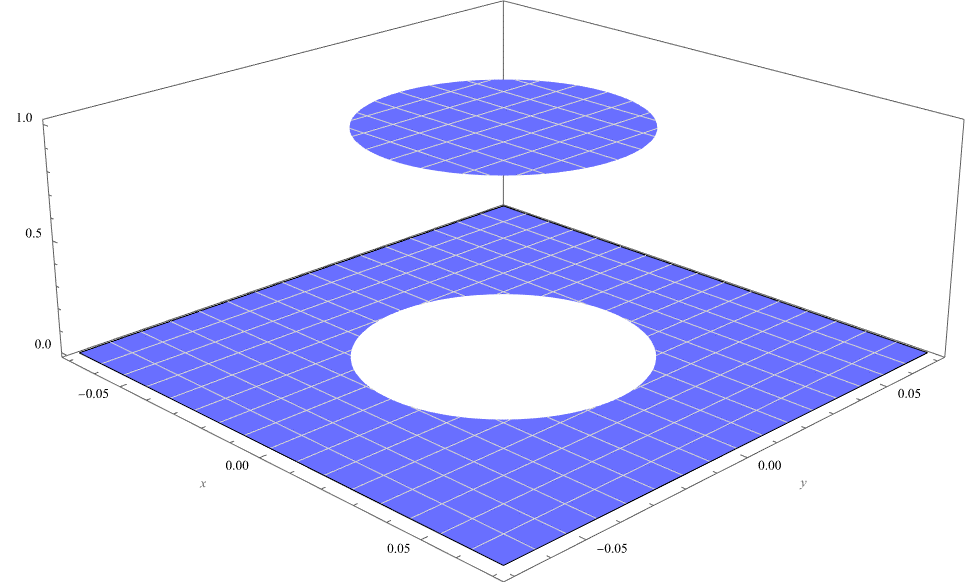
\includegraphics[width=.7\textwidth]{figures/stepfunction.png}
    \caption{\it 3D graph of the Heaviside step function defined over $\Omega$}
    \label{fig:fig_4_2}
\end{figure}
\\
\normalsize{\indent To validate the coefficient $k=519,69 \ m^{-2}$, it is possible to now integrate in Cartesian coordinates but on a disk. As said previously, the idea is to project the values of a function $f$ on a non-zero area $\Omega$ defined by $H_\Omega$, this is written as follows:}
\\
\begin{equation}
    \int\displaylimits_{\Omega_{cyl}} f \ rdrd\theta = \int\displaylimits_{\Omega_{car}} \proj{f}{H_\Omega} \ dxdy
\end{equation}
\\
\normalsize{with $\Omega_{cyl}$ being the cylindrical integration limits and $\Omega_{cyl}$ the cartesian integration limits. The fully written and calculated integral is :}
\\
\begin{equation}
    k \int\displaylimits_{-a}^{a} \int\displaylimits_{-b}^{b} \proj{\exp\left(-2\left(\frac{x+y}{35[mm]}\right)^2 \right)}{H(35[mm]^2 - x^2 - y^2 )} \ dxdy = 0,867
\end{equation}
\\
\normalsize{\indent The value of the integral is correct, and the integration coefficient for the Cartesian coordinates heat flux distribution is $q_0=473957 \ Wm^{-2}$,  which is the same as the cylindrical one. This is a good sight since the distribution are defined to be the same, it is reassuring to get the same result. For the elliptical one, the method is the same as the circular one except the argument in the Heaviside step function \eqref{eqn:HSF} isn’t derived for the circle equation but from the ellipse equation. The function for axisymmetric heat flux distribution written in cartesian coordinates is \eqref{eqn:carCSGHD}:}
\\
\begin{equation}
    \color{red}\boxed{\color{black} f_{axisym.}^{car. CS}(x,y) = 473957 \exp\left(-2\left(\frac{x+y}{35[mm]}\right)^2 \right) [W/m^2]}
    \label{eqn:carCSGHD}
\end{equation}
\\
\normalsize{\indent For the calculation of the non-axisymmetric integration coefficient (semi-minor radius of $35 \ mm$ and semi-major radius of $68 \ mm$), it is possible to proceed the same way as above. The ellipse is defined via the ellipse equation $(\frac{x}{a})^2 + (\frac{y}{b})^2 = 1$ with $a$ and $b$ being respectively the minor semi-radius and major semi-radius. The Heaviside step function \eqref{eqn:HSF} is written $H\left(1 - \left(\frac{x}{a}\right)^2 - \left(\frac{y}{b}\right)^2 \right)$. The normalization of the integral as well as the calculation of the integral on the ellipse is done the same way as before. The function on which the distribution $f$ is projected is the Heaviside step function \eqref{eqn:HSF} defined on an ellipse. The projection $\proj{f}{H_{\Omega}}$ is integrated and the results yields a normalization coefficient $k_{norm}$ of $267,5 \ m^{-2}$ and an integration coefficient $q_0$ of $243948 \ W/m^{2}$. The function for non-axisymmetric heat flux distribution written in cartesian coordinates is \eqref{eqn:carCSGHDNA}:}
\\
\begin{equation}
    \color{red}\boxed{\color{black} f_{non-axisym.}^{car. CS}(x,y) = 243948 \exp\left(-2\left(\left(\frac{x}{35[mm]}\right)^2 + \left(\frac{y}{68[mm]}\right)^2 \right) \right) [W/m^2]}
    \label{eqn:carCSGHDNA}
\end{equation}
\\
\normalsize{\indent All integration coefficients as well as the standard deviations of the distributions are summarized below:}

% INSERT THE SUMMARY TABLE

\subsection{Calculation of the surface integrales}